\documentclass[a4paper, 10pt, final, garamond]{book}
\usepackage{cours-preambule}
\graphicspath{{./figures/}}
\addto\captionsfrench{\renewcommand{\figurename}{Fig.}}

\makeatletter
\renewcommand{\@chapapp}{Contr\^ole de connaissances}
\makeatother

% \toggletrue{student}
% \toggletrue{corrige}
\renewcommand{\mycol}{black}
% \renewcommand{\mycol}{gray}

\hfuzz=5.003pt

\begin{document}
\setcounter{chapter}{14}

\settype{enon}
\settype{solu}

\chapter{Dynamique du point et mouvements courbes\ifstudent{~(15')}}

\begin{enumerate}[label=\sqenumi]
	\item[n]{3}%
	      Énoncer les trois lois de \textsc{Newton}. On travaille avec un système
	      ouvert.
	      \smallbreak
	      \vspace{-15pt}
	      \psw{%
		      \begin{enumerate}
			      \item[l][20]{\protect\pt{1}}
			            $\exists \Rc$ galiléens $: (\forall \Mr ~|~ \sum
				            \Ff_{\ext\to\Mr} =
				            \of)$, $\Mr$ est soit au repos, soit en translation
			            rectiligne uniforme~;
			      \item[l][20]{\protect\pt{1}} $\dv{\pf\Rg(\Mr)}{t} = \sum
				            \Ff_{\ext\to\Mr}$~;
			      \item[l][20]{\protect\pt{1}} $\forall (\Mr_1,\Mr_2), \Ff_{1\to2} =
				            -\Ff_{2\to 1}$.
		      \end{enumerate}
	      }%
	\item[n]{7}%
	      Établir la longueur d'équilibre d'un ressort vertical. Porter une
	      attention particulière à l'établissement du système d'étude.
	      \smallbreak
	      \vspace{-15pt}
	      \noindent
	      \begin{minipage}[t]{0.75\linewidth}
		      % \vspace{-60pt}
		      \psw{
			      \begin{enumerate}[label=\sqenumi]
				      \item[b]{\ltm[20]{\pt{1}}Système}~:
				            \{masse\} M ($m$) dans $\Rc\ind{labo}$ supposé
				            galiléen.
				      \item[b]{\ltm[20]{\pt{1}}Schéma}~: cf. Figure~15.1.
				      \item[b]{\ltm[20]{\pt{1}}Modélisation}~:
				            repère $(\Or, \uz)$, repérage~: $\OM = -\ell\uz$, $\vf =
					            -\lp\uz$, $\af = -\lpp\uz$.
			      \end{enumerate}
		      }
	      \end{minipage}
	      \hfill
	      \begin{minipage}[t]{.25\linewidth}
		      \vspace*{0pt}
		      \begin{center}
			      \sswitch{
				      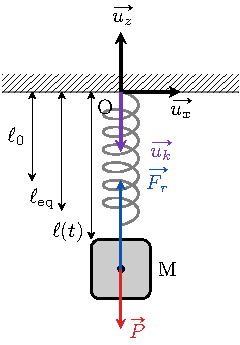
\includegraphics[width=.7\linewidth,
					      draft=true]{ressort_vert_prof}
			      }{
				      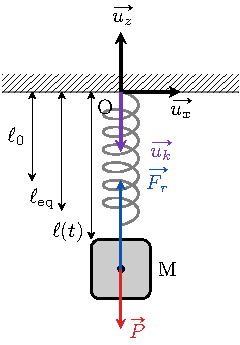
\includegraphics[width=.7\linewidth]{ressort_vert_prof}
			      }
			      \captionof{figure}{}
		      \end{center}
	      \end{minipage}
	      \vspace{-90pt}
	      \psw{
		      \begin{enumerate}[label=\sqenumi, start=4]
			      \item[b]{BdF}~:
			            \vspace{-15pt}
			            \[
				            \begin{array}{ll}
					            \pt{1}\textbf{Poids}                & \Pf = m\gf = -mg\uz       \\
					            \pt{1}\textbf{Force \textsc{Hooke}} & \Ff = k(\ell - \ell_0)\uz
				            \end{array}
			            \]
			      \item[b]{PFD à l'équilibre}~:
			            \vspace{-22pt}
			            \begin{gather*}
				            \of \stm[-1]{=} \sum \Ff\ind{ext}
				            \Lra
				            0 = -mg + k(\ell_{\eql} - \ell_0)
				            \\\Lra
				            k(\ell_{\eql} - \ell_0) = mg
				            \Lra
				            \boxed{\ell_{\eql} \stm[-1]{=} \ell_0 + \frac{mg}{k}}
			            \end{gather*}
		      \end{enumerate}
	      }
	\item[n]{8}%
	      Représenter sur un schéma les coordonnées cylindriques. Détaillez les
	      projections de $\ur$ et $\ut$ sur la base cartésienne, donner
	      l'expression de $\OM$ et $\dd{\OM}$ \xul{sans démonstration}, et
	      \textbf{démontrer les expressions} de $\vf$ et $\af$ \xul{sans démontrer
		      les expressions de $\dv{\ur}{t}$ et $\dv{\ut}{t}$}.
	      \smallbreak
	      \noindent
	      \begin{minipage}[t]{.70\linewidth}
		      \psw{
			      \begin{gather*}
				      \beforetext{\pt{1}}
				      \ur = \cos(\th)\ux + \sin(\th)\uy \qet \ur = -\sin(\th)\ux +
				      \cos(\th)\uy \\
				      \beforetext{\pt{1}}
				      \OM(t) = r(t)\ur + z(t) \uz \\
				      \beforetext{\pt{1}}
				      \dd{\OM} = \dd{r}\ur + r \dd{\th}\ut + \dd{z}\uz
				      \\
				      \beforetext{\pt{1}}
				      \vf(t) = \dv{\OM}{t} = \rp\ur + r \tp \ut + \zp\uz
				      \\
				      \af(t) =
				      \dv{\tikzmark{DV}}{t}
				      \left(
				      \rp\tikzmark{RP}\ur\tikzmark{UR} +
				      r\tikzmark{R}\tp\tikzmark{TP}\ut\tikzmark{UT} +
				      \zp\tikzmark{ZP}\uz
				      \right)
				      \Lra
				      \af(t) \stm{=}
				      \psw[orchid]{\rpp}\ur +
				      \rp \psw[cornflowerblue]{\dv{\ur}{t}} +
				      \psw[limegreen]{\rp}\tp\ut +
				      r\psw[orange]{\tpp}\ut +
				      r\tp \psw[firebrick]{\dv{\ut}{t}} +
				      \zpp\uz
				      \\\Lra
				      \boxed{
					      \af(t) \stm[-1]{=} \left( \rpp -r\tp^2 \right)\ur +
					      \left( 2\rp\tp + r\tpp \right)\ut +
					      \zpp\uz
				      }
			      \end{gather*}
			      \tikz[remember picture, overlay]
			      \draw[-stealth, transform canvas={yshift=6pt},
				      color=\sswitch{white}{orchid}]
			      (pic cs:DV) to [out=90, in=90] ([shift={(-3pt,3pt)}]pic cs:RP)
			      ; \tikz[remember picture, overlay]
			      \draw[-stealth, transform canvas={yshift=6pt},
				      color=\sswitch{white}{cornflowerblue}]
			      (pic cs:DV) to [out=90, in=90] ([shift={(-6pt,6pt)}]pic cs:UR)
			      ; \tikz[remember picture, overlay]
			      \draw[-stealth, transform canvas={yshift=6pt},
				      color=\sswitch{white}{limegreen}]
			      (pic cs:DV) to [out=90, in=90] ([shift={(-3pt,3pt)}]pic cs:R)
			      ; \tikz[remember picture, overlay]
			      \draw[-stealth, transform canvas={yshift=6pt},
				      color=\sswitch{white}{orange}]
			      (pic cs:DV) to [out=90, in=90] ([shift={(-3pt,6pt)}]pic cs:TP)
			      ; \tikz[remember picture, overlay]
			      \draw[-stealth, transform canvas={yshift=6pt},
				      color=\sswitch{white}{firebrick}]
			      (pic cs:DV) to [out=90, in=90] ([shift={(-6pt,6pt)}]pic cs:UT)
			      ; \tikz[remember picture, overlay]
			      \draw[-stealth, transform canvas={yshift=6pt},
				      color=\sswitch{white}{black}]
			      (pic cs:DV) to [out=90, in=90] ([shift={(-3pt,3pt)}]pic cs:ZP)
			      ;
		      }
	      \end{minipage}
	      \hfill
	      \begin{minipage}[t]{.20\linewidth}
		      \vspace*{0pt}
		      \begin{center}
			      \sswitch{
				      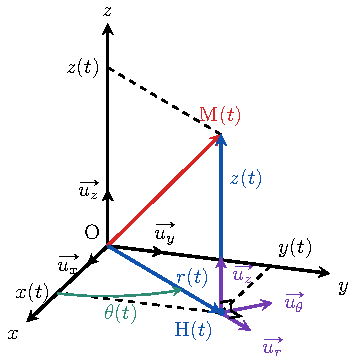
\includegraphics[width=\linewidth, draft=true]{pos_cyl_prof}
			      }{
				      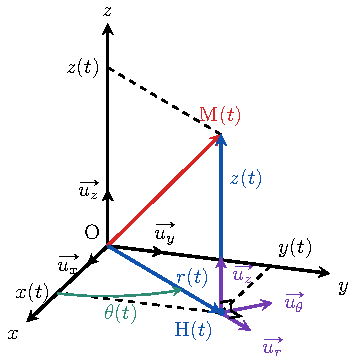
\includegraphics[width=\linewidth]{pos_cyl_prof}
			      }
			      \vspace{-15pt}
			      \captionsetup{justification=centering}
			      \captionof{figure}{\smallbreak
				      Cylindriques\protect\pt{1}\protect\pt{1}}
		      \end{center}
	      \end{minipage}
	\item[n]{4}%
	      \noindent
	      \begin{minipage}[t]{.70\linewidth}
		      Effectuez le bilan des forces et appliquer le PFD grâce à la question
		      précédente, que vous simplifierez dans les conditions de l'exercice.
		      Sous quelle condition l'une des 2 équations différentielles obtenues
		      est celle d'un oscillateur harmonique~?
		      \smallbreak
		      \psw{%
			      \begin{gather*}
				      \pt{1}
				      \begin{array}{ll}
					      \textbf{Poids}   & \Pf = m\gf = mg(\cos\th \ur - \sin\th \ut)
					      \\
					      \textbf{Tension} & \Tf = -T\ur
				      \end{array}
				      \\
				      \beforetext{Or,}
				      m\af \stm[-1]{=} m (-\ell\tp^2 \ur + \ell\tpp \ut) = \Pf + \Tf
			      \end{gather*}
			      \begin{empheq}[box=\fbox, left=\stm{\Lra}\empheqlbrace]{align}
				      mg\cos\th + m \ell\tp^2 & = T
				      \notag\\
				      \label{eq:pendb}
				      m \ell\tpp + mg\sin\th & = 0
			      \end{empheq}
			      L'équation~(15.1) est l'équation d'un oscillateur harmonique pour
			      des petits angles ($\sin(\theta) \Sim_{\th\to0} \th$)\pt{1}.
		      }%
	      \end{minipage}
	      \hfill
	      \begin{minipage}[t]{0.25\linewidth}
		      \vspace*{0pt}
		      \begin{center}
			      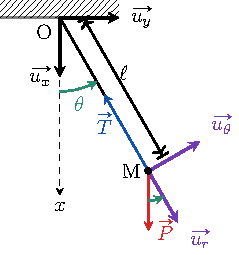
\includegraphics[width=\linewidth]{pendule_prof}
			      \captionof{figure}{Schéma}
			      \label{fig:pendule}
		      \end{center}
	      \end{minipage}
	      \ifstudent{
		      \begin{tikzpicture}[remember picture, overlay]
			      \node[anchor=north west, align=left]
			      at ([shift={(1.4cm,0)}]current page.north west)
			      {\\[5pt]\Large\bfseries \textsc{Nom}~:\\[10pt]\Large\bfseries
				      Prénom~:};
			      \node[anchor=north east, align=right]
			      at ([shift={(-1.5cm,-17pt)}]current page.north east)
			      {\Large\bfseries Note~:\hspace{1cm}/20};
		      \end{tikzpicture}
	      }
\end{enumerate}
\end{document}
